\documentclass[a4paper, 8pt]{extarticle}
% (1) Encoding, Fonts, and Layout
\usepackage[T1]{fontenc}
\usepackage{lmodern}
\usepackage[margin=1in]{geometry}


% (2) Common Packages
\usepackage{amsmath, amssymb, amsthm}
\usepackage{xcolor}
\usepackage{caption}
\usepackage{tikz}
\usepackage{pgfplots}
\pgfplotsset{compat=newest}
\usepackage{etoolbox}
\usepackage{tikz-3dplot}
\tdplotsetmaincoords{75}{120}
\usepackage[inline]{enumitem}
\usepackage{bookmark}
\usepackage{mathtools}
\usepackage{subcaption} % For subfigures
\usepackage[normalem]{ulem} % For better underline commands

% Micro-typography
\usepackage{microtype}

% Patching pgfplots warning
\makeatletter
\patchcmd{\pgfplots@applistXXpushback@smallbuf}{\pgfplots@error}{\pgfplots@warning}{}{}
\makeatother

% (3) tcolorbox and Theorem Libraries
\usepackage{tcolorbox}
\tcbuselibrary{theorems}

% (4) Define Colors
\definecolor{custom_green}{HTML}{a3be8c}
\definecolor{custom_red}{HTML}{dc322f}
\definecolor{custom_blue}{HTML}{268bd2}
\definecolor{custom_purple}{HTML}{b48ead}

\definecolor{base}{HTML}{eceff4}
\definecolor{gray1}{HTML}{e5e9f0}
\definecolor{gray2}{HTML}{d8dee9}
\definecolor{gray3}{HTML}{2e3440}
\pagecolor{base}

% (5) Custom tcolorbox Environments
\newtcolorbox{definitionbox}[1][]{
    title=\textbf{Definition} {#1},
    fonttitle=\bfseries\boldmath,
    arc=0mm,
    bottomtitle=0.5mm,
    boxrule=0mm,
    colbacktitle=gray2,
    colback=gray1,
    coltitle=gray3,
    coltext=gray3,
    left=2.5mm,
    leftrule=1mm,
    rightrule=1mm,
    right=3.5mm,
    toptitle=0.75mm,
    colframe=custom_red,
}

\newtcolorbox{proofbox}{
    title=\textbf{Proof},
    fonttitle=\bfseries\boldmath,
    arc=0mm,
    bottomtitle=0.5mm,
    boxrule=0mm,
    colbacktitle=gray2,
    colback=gray1,
    coltitle=gray3,
    left=2.5mm,
    leftrule=1mm,
    rightrule=1mm,
    right=3.5mm,
    toptitle=0.75mm,
    colframe=custom_blue,
    coltext=gray3,
}

\newtcolorbox{theorembox}[1][]{
    title=\textbf{Theorem} {#1},
    fonttitle=\bfseries\boldmath,
    arc=0mm,
    bottomtitle=0.5mm,
    boxrule=0mm,
    colbacktitle=gray2,
    colback=gray1,
    coltitle=gray3,
    left=2.5mm,
    leftrule=1mm,
    rightrule=1mm,
    right=3.5mm,
    toptitle=0.75mm,
    colframe=custom_green,
    coltext=gray3
}

\newtcolorbox{notebox}{
    title=\textbf{Note},
    fonttitle=\bfseries\boldmath,
    arc=0mm,
    bottomtitle=0.5mm,
    boxrule=0mm,
    colbacktitle=gray2,
    coltitle=gray3,
    left=2.5mm,
    leftrule=1mm,
    rightrule=1mm,
    right=3.5mm,
    toptitle=0.75mm,
    colframe=custom_blue,
    coltext=gray3
}

\newtcolorbox{examplebox}[1][]{
    title=\textbf{Example} {#1},
    fonttitle=\bfseries\boldmath,
    arc=0mm,
    bottomtitle=0.5mm,
    boxrule=0mm,
    colbacktitle=gray2,
    colback=gray1,
    coltitle=gray3,
    left=2.5mm,
    leftrule=1mm,
    rightrule=1mm,
    right=3.5mm,
    toptitle=0.75mm,
    colframe=gray3,
    fontupper=\footnotesize,
    coltext=gray3
}

% (6) Theorem Environments
\theoremstyle{definition}
\newtheorem{definition}{Definition}[section]
\newtheorem{example}[definition]{Example}

\theoremstyle{plain}
\newtheorem{theorem}[definition]{Theorem}

% (7) Hyperlinks
\usepackage{hyperref}
\hypersetup{
    colorlinks=true,    % Use colored text for links
    linkcolor=custom_red,      % Set link text color to red
    pdfborder={0 0 0}   % Remove the default box around links
}

% macros.tex
\newcommand{\intinf}{\int_0^{\infty}} % Integral from 0 to infinity
\newcommand{\diff}[2]{\frac{d#1}{d#2}} % Derivative


\title{
\textbf{MA2287: Complex Analysis Exam Notes} \\ 
}


\author{
  Robert Davidson
}   

 

\date{} % Empty date

\begin{document}

\maketitle
\pagebreak
\tableofcontents
\pagebreak


\section{Question 1: }
\subsection{Sketch the region in the complex plane determined by the inequality}
\begin{itemize}
    \item $|z - 4| > 3|z+4|$ \hfill \hyperref[sol:2023Q1a]{\uline{2023 Q1(a)}}
    \item $\{ z \in \mathbb{C} : |2z - 1| < 2|2z-i|$\} \hfill  \hyperref[sol:2022Q1a]{\uline{2022 Q1(a), 2021 Q1(d), 2017 Q1(a), 2016 Q1(a)}}
\end{itemize}
\subsection{Determine all solutions to roots of unity}
\begin{itemize}
    \item $z^6 -1 = 0$ and factorize $x^6 -1$ as a product of linear and quadratic factors \hfill \hyperref[sol:2023Q1b]{\uline{2023 Q1(b),2021 Q1(c)}}
    \item $z^4 = -81i$ and find a polynomial $p(z)$ with complex coefficients with root $w$ and $p(\overline{w}) \neq 0$ \hfill 2022 Q1(b), \hyperref[sol:20188Q1b]{\uline{2018 Q1(b)}}
    \item $z^3 = 1+i$, let $n \in \mathbb{N}$ and $w \neq 1$ be an n-th root of unity. Prove $1 + w + w^2 + \ldots + w^{n-1} = 0$ \hfill 2016 Q1(c)
\end{itemize}
\subsection{Determine and sketch the image under the mapping}
\begin{itemize}
    \item $w = e^z$, $\{z \in \mathbb{C} : \pi / 4 \leq \text{Im}(z) \leq \pi /2\}$ \hfill 2023 Q1(c), 2021 Q1(a), 2017 Q1(d)
    \item $w = \text{Log}(z)$, $\{z: |z| > 1, 0 \leq \text{Arg}(z) \leq \pi / 2\}$ \hfill 2022 Q1(d), 2018 Q1(d), 2016 Q1(d)
\end{itemize}
\subsection{Find z where the function is 0}
\begin{itemize}
    \item $\cos(z) = \frac{e^{iz} + e^{-iz}}{2}$ \hfill 2022 Q1(d)
\end{itemize}
\subsection{Calculate principal value Log(z)}
\begin{itemize}
    \item z = $-\frac{1}{\sqrt{2}} + \frac{1}{\sqrt{2}} i$ and prove $e^z$ is the inverse function of Log(z) \hfill 2022 Q1(c), 2018 Q1(c), 2017 Q1(c)
\end{itemize}
\subsection{Prove the following}
\begin{itemize}
    \item Define the complex conjugate ($\overline{w}$) and prove if $w$ is a zero of a polynomial $p(z)$ = $a_0 + a_1 z + \ldots + a_n z^n$ then $\overline{w}$ is also a zero of $p(z)$ \hfill 2021 Q1(b), 2018 Q1(a), 2016 Q1(b)
    \item Define the complex exponential function $e^z$ and prove Eulers Formula $e^{i \theta} = \cos(\theta) + i \sin(\theta)$ \hfill 2017 Q1(b)
\end{itemize}





\pagebreak


\section{Question 2: }
\subsection{Determine image of the line}
\begin{itemize}
    \item $f(z) = \frac{1}{z} \quad \{z \in \mathbb{C}: \text{Re}(z) = 2\}$ \hfill 2023 Q2(a), 2021 Q2(b)
    \item $f(z) = \frac{1}{z} \quad \{z \in \mathbb{C}: \text{Re}(z) = 1\}$ \hfill 2022 Q2(a), 2018 Q2(a), 2017 Q2(a)
\end{itemize}
\subsection{State and Use Cauchy-Riemann Equations}
\begin{itemize}
    \item State CRE, and use to prove $f(z) = \frac{1}{z}$ is holomoprhic on $\mathbb{C} \backslash \{0\}$ \hfill 2023 Q2(a)
    \item State CRE, and use to prove $f(z) = z^2$ is holomoprhic on $\mathbb{C}$ \hfill 2022 Q2(b)
    \item State CRE. Let $f = u+iv$ be holomoprhic on $\Omega \subset \mathbb{C}$. Prove $\nabla u$ and $\nabla v$ are perpendicular of equal length \hfill 2016 Q2(b)
\end{itemize}
\subsection{Show that}
\begin{itemize}
    \item If $\overline{f(z)} = f(\overline{z})$ for all $z \in \mathbb{C}$ then $f(x)$ is real for all $x \in \mathbb{R}$. And if in addition $f$ is holomoprhic at $x \in \mathbb{R}$ then $f'(x)$ is real. \hfill 2023 Q2(c)
    \item Define that is meant for a function $g$ to be harmonic. If $f = u +iv$ is holomoprhic on $\Omega \subset \mathbb{C}$, prove that $v(x,y)$ is a harmonic function, and that $\nabla u$ and $\nabla v$ are perpendicular of equal length. \hfill 2022 Q2(c), 2018 Q2(b)
    \item If $\overline{f(z)} = f(\overline{z})$ for all $z \in \mathbb{C}$ then $f(x)$ is real for all $x \in \mathbb{R}$. And if in addition $f$ is holomoprhic at $0$ then the function $f'(0)$ is real.\hfill 2021 Q2(a), 2017 Q2(c)
    \item Let $f(z) = u +iv$ be holomoprhic on an open subset $\Omega$ of the complex plane and let $h(u,v)$ be a harmonic function of $u$ and $v$ on $f(\Omega)$. Prove that $g(x,y) = h(u(x,y), v(x,y))$ is harmonic on $\Omega$ (You may assume $\nabla u, \nabla v$ are equal length and perpendicular)\hfill 2021 Q2(c)
    \item Define what is meant for a function $f(z)$ to be holomoprhic at a point $z_0 \in \mathbb{C}$ and prove that $f(z) = z^2$ is holomoprhic and find its derivative there. Hence prove that the product $uv$ is harmonic where $f=u +iv$ \hfill 2018 Q2(c)
    \item Define what is meant for a function $f(z)$ to be holomoprhic at a point $z_0 \in \mathbb{C}$ and prove that $f(z) = \frac{1}{z}$ is holomoprhic on $\mathbb{C} \backslash 0$ and find its derivative there (State any theorems used) \hfill 2017 Q2(b)
    \item Let $h(u,v)$ be a harmonic function of $u, v$ on $f(\Omega)$ (See 2016 Q2(b)). Prove that $g(x,y) = h(u(x,y), v(x,y))$ is harmonic on $\Omega$ \hfill 2016 Q2(c)
\end{itemize}
\subsection{Find Mobius Transformation}
\begin{itemize}
    \item $T(z) : (-1, 1, \infty) \mapsto (-1, -i, 1)$ \hfill 2023 Q2(d)
    \item $T(z) : (2, 1, -1) \mapsto (1, 0, \infty)$    \hfill 2022 Q2(d)
    \item $T(z) : (-i, -1, 1) \mapsto (1, 0, \infty)$ and find the inverse Mobius Transformation \hfill 2021 Q2(d)
    \item $T(z) : (-i, -1, i) \mapsto (1, 0, \infty)$ and find the inverse Mobius Transformation \hfill 2018 Q2(d), 2017 Q2(d)
    \item $T(z) : (-1, \frac{1}{2}, 2) \mapsto (1, 0, \infty)$ and find the inverse Mobius Transformation \hfill 2016 Q2(d)
\end{itemize}

\pagebreak

\section{Worked Examples - Q1}

\begin{examplebox}[2023 Q1(a)]
    \phantomsection
    \label{sol:2023Q1a}

    \textbf{Given} $|z - 4| > 3|z+4|$ \\
    \textbf{Write} $\boldsymbol{z = x + iy}$
    \begin{align*}
        | x + iy -4|         & > 3 |x + iy + 4|         \\
        | (x - 4) + iy|      & > 3 |(x + 4) + iy|       \\
        \sqrt{(x-4)^2 + y^2} & > 3 \sqrt{(x+4)^2 + y^2} \\
    \end{align*}
    \textbf{Square both sides}
    \begin{align*}
        (x-4)^2 + y^2                                 & > 9((x+4)^2 + y^2)                                                         \\
        (x^2 - 8x + 16 + y^2)                         & > 9x^2 + 72x + 144 + 9y^2                                                  \\
        x^2 - 8x + 16 + y^2 - 9x^2 - 72x - 144 - 9y^2 & > 0                       & \emph{Moving all terms to one side}            \\
        -8x^2 - 80x - 8y^2 - 128                      & > 0                       & \emph{Simplify }                               \\
        x^2 + 10x + y^2 - 16                          & < 0                       & \emph{Dividing by -8 and reversing inequality} \\
    \end{align*}

    \textbf{Focus on x and complete the square}
    \begin{align*}
        x + bx                   = \left(x + \frac{b}{2}\right)^2 - \left(\frac{b}{2}\right)^2 & \Rightarrow  x^2 + 10x = (x + 5)^2 - 25 & \emph{Complete the square}             \\
        (x+5)^2 - 25 + y^2 + 16                                                                & < 0                                     & \emph{Substitute back into inequality} \\
        (x+5)^2 + y^2 + 9                                                                      & < 0                                     & \emph{Simplify}                        \\
        (x+5)^2 + y^2                                                                          & < -9                                    & \emph{Subtract 9}                      \\
    \end{align*}

    \begin{minipage}{0.49\textwidth}
        \textbf{Recall the eqation of a circle}
        $$(x - a)^2 + (y - b)^2 = r^2 \Rightarrow  (x+5)^2 + y^2 < -9  $$
        \textbf{Therefore the region is all the points inside circle with radius 3 and center at (-5, 0)}
    \end{minipage}
    \begin{minipage}{0.5\textwidth}
        \begin{center}
            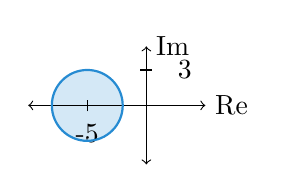
\begin{tikzpicture}[scale=0.15]
                \fill[custom_blue!20, even odd rule] (-5,0) circle [radius=3];
                \draw[<->] (-10, 0) -- (5, 0) node[right] {$\text{Re}$};
                \draw[<->] (0, -5) -- (0, 5) node[right] {$\text{Im}$};
                \draw (-5,-0.5) -- (-5,0.5) node[below=0.2cm] {-5};
                \draw (-0.5,3) -- (0.5,3) node[right=0.2cm] {3};
                \draw[custom_blue, thick]{(-5, 0) circle [radius=3]};

            \end{tikzpicture}
        \end{center}
    \end{minipage}
\end{examplebox}
\begin{examplebox}[2022 Q1(a), 2021 Q1(d), 2017 Q1(a), 2016 Q1(a)]
    \phantomsection
    \label{sol:2022Q1a}
    \textbf{Given} $\{ z \in \mathbb{C} : |2z - 1| < 2|2z-i|\}$ \\
    \textbf{Write} $z = x + iy$
    \begin{align*}
        |2x + i2y -1 |                                        & < 2 |2x + i2y - i|                                                        \\
        |(2x -1) + i2y|                                       & < 2 |2x + i(2y -1)|                                                       \\
        \sqrt{(2x-1)^2 + 4y^2}                                & < 2 \sqrt{4x^2 + (2y-1)^2}                                                \\
        (2x-1)^2 + 4y^2                                       & < 4[4x^2 + (2y-1)^2]       & \emph{Square both sides}                     \\
        4x^2 - 4x + 1 + 4y^2                                  & < 16x^2 + 16y^2 -16y +4    & \emph{Expand}                                \\
        -12x^2 - 4x - 12y^2 + 16y -3                          & < 0                        & \emph{Move all terms to one side}            \\
        12x^2 + 4x + 12y^2 - 16y + 3                          & > 0                        & \emph{Multiply by -1 and reverse inequality} \\
        x^2 + \frac{1}{3}x + y^2 - \frac{4}{3}y + \frac{1}{4} & > 0                        & \emph{Divide by 12}                          \\
    \end{align*}
    \textbf{Complete square for x}
    $$x^2 + bx = \left(x + \frac{b}{2}\right)^2 - \left(\frac{b}{2}\right)^2 \Rightarrow x^2 + \frac{1}{3}x = \left(x + \frac{1}{6}\right)^2 - \left(\frac{1}{36}\right)$$
    \textbf{Complete square for y}
    $$y^2 + by = \left(y - \frac{2}{3}\right)^2 - \left(\frac{4}{9}\right)$$
    \textbf{Substitute back into inequality}
    \begin{align*}
        \left(x + \frac{1}{6}\right)^2 - \left(\frac{1}{36}\right) + \left(y - \frac{2}{3}\right)^2 - \left(\frac{4}{9}\right)  + \frac{1}{4} & > 0            & \emph{Substitute back into inequality}   \\
        \left(x + \frac{1}{6}\right)^2 + \left(y - \frac{2}{3}\right)^2                                                                       & >  \frac{2}{9} & \emph{Simplify and move constant across} \\
    \end{align*}

    \begin{minipage}{0.49\textwidth}
        \textbf{Recall the eqation of a circle}
        $$(x - a)^2 + (y - b)^2 = r^2 \Rightarrow  \left(x+ \frac{1}{6}\right)^2 + \left(y - \frac{2}{3}\right)^2 < \frac{2}{9}  $$
        \textbf{Therefore the region is all the points OUTSIDE the circle with radius $\frac{\sqrt{2}}{3}$ and center at $(-\frac{1}{6}, \frac{2}{3})$}
    \end{minipage}
    \begin{minipage}{0.5\textwidth}
        \begin{center}
            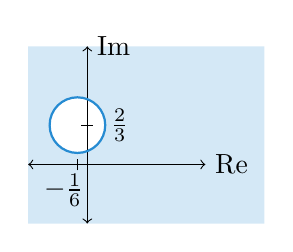
\begin{tikzpicture}[scale=0.75]
                \fill[custom_blue!20, even odd rule]
                (-1,-1) rectangle (3,2)
                (-0.167,0.666) circle [radius=0.471];
                \draw[<->] (-1, 0) -- (2, 0) node[right] {$\text{Re}$};
                \draw[<->] (0, -1) -- (0, 2) node[right] {$\text{Im}$};
                \draw (-0.167,-0.1) -- (-0.167,0.1) node[below=0.4cm, left=-0.2cm] {$-\frac{1}{6}$};
                \draw (-0.1,0.66) -- (0.1,0.66) node[right=0.1cm] {$\frac{2}{3}$};
                \draw[custom_blue, thick]{(-0.167, 0.666) circle [radius=0.471]};
            \end{tikzpicture}
        \end{center}
    \end{minipage}
\end{examplebox}
\begin{examplebox}[Determine all solutions to $z^6 -1 = 0$ and factor $x^6-1$ as a product of linear and quadratic factors]
    \phantomsection
    \label{sol:2023Q1b}
    \textbf{Given} $z^6 -1 = 0$ \\
    \textbf{Write} $z = e^{i \theta}$ and $1 = e^{i 2 \pi k}$ for $k \in \mathbb{Z}$

    \begin{align*}
        z^6 -1                         & = 0               \\
        e^{i 6 \theta} - e^{i 2 \pi k} & = 0               \\
        e^{i 6 \theta}                 & = e^{i 2 \pi k}   \\
        6 \theta                       & = 2 \pi k         \\
        \theta                         & = \frac{\pi k}{3} \\
    \end{align*}
    \textbf{Therefore the solutions are}
    $$z = e^{i \theta} = e^{i \frac{\pi k}{3}} = \cos\left(\frac{\pi k}{3}\right) + i\sin\left(\frac{\pi k}{3}\right) \quad \text{for} \quad k = 0, 1, 2, 3, 4, 5$$

    \begin{minipage}{0.49\textwidth}
        \begin{align*}
            k = 0 : w_0 =  & \cos\left(0\right) + i\sin\left(0\right) = 1 + i0                                                       \\
            k = 1 : w_1 =  & \cos\left(\frac{\pi}{3}\right) + i\sin\left(\frac{\pi}{3}\right)    = \frac{1}{2} + i\frac{\sqrt{3}}{2} \\
            k = 2 : w_2  = & \cos\left(\frac{2\pi}{3}\right) + i\sin\left(\frac{2\pi}{3}\right) = -\frac{1}{2} + i\frac{\sqrt{3}}{2} \\
            k = 3 : w_3 =  & \cos\left(\pi\right) + i\sin\left(\pi\right)                        = -1                                \\
            k = 4 : w_4 =  & \cos\left(\frac{4\pi}{3}\right) + i\sin\left(\frac{4\pi}{3}\right) = -\frac{1}{2} - i\frac{\sqrt{3}}{2} \\
            k = 5 : w_5 =  & \cos\left(\frac{5\pi}{3}\right) + i\sin\left(\frac{5\pi}{3}\right) = \frac{1}{2} - i\frac{\sqrt{3}}{2}  \\
        \end{align*}
    \end{minipage}
    \begin{minipage}{0.5\textwidth}
        \begin{center}
            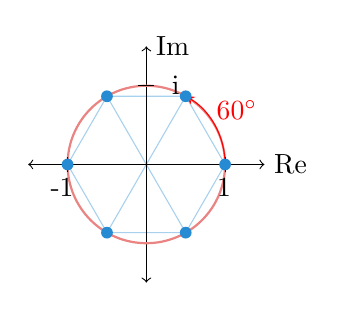
\begin{tikzpicture}
                \draw[custom_blue!40] (-1, 0) -- (-0.5, 0.866) -- (0.5, 0.866) -- (1, 0) -- (0.5, -0.866) -- (-0.5, -0.866) -- (-1, 0);
                \draw[custom_blue!40] (0, 0) -- (1, 0);
                \draw[custom_blue!40] (0, 0) -- (0.5, 0.866);
                \draw[custom_blue!40] (0, 0) -- (-0.5, 0.866);
                \draw[custom_blue!40] (0, 0) -- (-1, 0);
                \draw[custom_blue!40] (0, 0) -- (-0.5, -0.866);
                \draw[custom_blue!40] (0, 0) -- (0.5, -0.866);

                \draw[<->] (-1.5, 0) -- (1.5, 0) node[right] {$\text{Re}$};
                \draw[<->] (0, -1.5) -- (0, 1.5) node[right] {$\text{Im}$};

                \draw[custom_red!60, thick] (0,0) circle [radius=1];

                \draw[->, red, >=stealth] (1,0) arc (0:60:1);
                \node[red, right=0.3cm, above=0.1cm] at (0.85,0.35) {$60^\circ$};

                \draw (1,-0.1) -- (1,0.1) node[below=0.4cm, left=-0.2cm] {1};
                \draw (-0.1,1) -- (0.1,1) node[right=0.1cm] {i};
                \draw (-1,-0.1) -- (-1,0.1) node[below=0.4cm, left=-0.2cm] {-1};

                \node at (1, 0) [custom_blue, circle, fill, inner sep=1.5pt]{};
                \node at (-1,0) [custom_blue, circle, fill, inner sep=1.5pt]{};
                \node at (0.5,0.866) [custom_blue, circle, fill, inner sep=1.5pt]{};
                \node at (-0.5,0.866) [custom_blue, circle, fill, inner sep=1.5pt]{};
                \node at (-0.5,-0.866) [custom_blue, circle, fill, inner sep=1.5pt]{};
                \node at (0.5,-0.866) [custom_blue, circle, fill, inner sep=1.5pt]{};
            \end{tikzpicture}
        \end{center}
    \end{minipage}

    \textbf{We can write:}
    $$x^6 -1 = (x - w_0)(x - w_1)(x - w_2)(x - w_3)(x - w_4)(x - w_5)$$
    \textbf{Rewriting to group complex conjugates}
    $$x^6 -1 = (z-w_0)(z-w_3) \cdot (z-w_1)(z-w_5) \cdot (z-w_2)(z-w_4)$$
    \textbf{Note that}
    \begin{align*}
        (w-z)(w-\overline{z}) & = w^2 - w\overline{z} - zw + z\overline{z} \\
                              & = w^2 - 2(\overline{z} + z) + 1
    \end{align*}
    \textbf{We recall that}
    \begin{align*}
        z = x + iy = e^{i\theta} = \cos(\theta) + i\sin(\theta)             \\
        \overline{z} = x - iy = e^{-i\theta} = \cos(\theta) - i\sin(\theta) \\
    \end{align*}
    \textbf{Then}
    \begin{align*}
        \overline{z} + z & = cos(\theta) + i\sin(\theta) + cos(\theta) - i\sin(\theta) \\
                         & = 2\cos(\theta)                                             \\
    \end{align*}
    \textbf{Thus}
    $$(w-z)(w-\overline{z})  = w^2 - 2\cos(\theta) + 1$$
    \begin{minipage}{0.49\textwidth}
        We see that $-\frac{5\pi}{3} = \frac{\pi}{3} - 2\pi$, thus:
        \begin{align*}
            (z-w_1)(z-w_5) & = (z - e^{i\frac{\pi}{3}})(z - e^{i\frac{5\pi}{3}}) \\
            (z-w_1)(z-w_5) & = z^2 - 2\cos\left(\frac{\pi}{3}\right) + 1         \\
            (z-w_1)(z-w_5) & = z^2 + z + 1
        \end{align*}
    \end{minipage}
    \begin{minipage}{0.5\textwidth}
        We see that $-\frac{4\pi}{3} = \frac{\pi}{3} - \pi$, thus:
        \begin{align*}
            (z-w_2)(z-w_4) & = (z - e^{i\frac{2\pi}{3}})(z - e^{i\frac{4\pi}{3}}) \\
            (z-w_2)(z-w_4) & = z^2 - 2\cos\left(\frac{2\pi}{3}\right) + 1         \\
            (z-w_2)(z-w_4) & = z^2 - z + 1
        \end{align*}
    \end{minipage}
    \textbf{Therefore}
    $$x^6 -1 = (x+1)(x-1)(x^2 + x + 1)(x^2 - x + 1)$$
\end{examplebox}

\begin{examplebox}[: Determine all solutions to $z^4 = -81i$ and find a polynomial $p(z)$ with complex coefficients with root $w$ and $p(\overline{w}) \neq 0$]
    \phantomsection
    \label{sol:20188Q1b}
    \textbf{Given} $z^4 = -81i$, we want to find $z^{4\left(\frac{1}{4}\right)} = w $ \\
    \textbf{Recall:}
    $$z^{1/n} = R^{1/n}[\cos\phi + i\sin \phi] \quad \text{with} \; \phi = \frac{\theta + 2k\pi}{n}, \; k \in (0,1,2,\dots, n-1) \quad \text{and} \; R = |z|$$
    \begin{minipage}{0.49\textwidth}
        \textbf{Thus}
        \begin{align*}
            R      & = \sqrt{0^2 + 81^2} = 81                                                                        \\
            \theta & = -\frac{\pi}{2}                                                                                \\
            \phi   & = \frac{\theta + 2k\pi}{n} = \frac{-\frac{\pi}{2} + 2k\pi}{4} = \frac{-\pi}{8} + \frac{k\pi}{2}
        \end{align*}
    \end{minipage}
    \begin{minipage}{0.5\textwidth}
        \begin{center}
            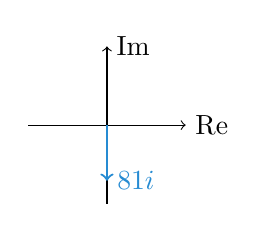
\begin{tikzpicture}
                \draw[->] (-1, 0) -- (1, 0) node[right] {$\text{Re}$};
                \draw[->] (0, -1) -- (0, 1) node[right] {$\text{Im}$};
                \draw[->, custom_blue, thick] (0,0) -- (0, -0.707) node[right] {$81i$};
            \end{tikzpicture}
        \end{center}
    \end{minipage}

    \textbf{Therefore}
    \begin{align*}
        w_k & = 81^{1/4}\left[\cos\left(\frac{-\pi}{8} + \frac{k\pi}{2}\right) + i\sin\left(\frac{-\pi}{8} + \frac{k\pi}{2}\right)\right] \quad k \in (0,1,2,3) \\
        w_0 & = 3\left[\cos\left(\frac{-\pi}{8}\right) + i\sin\left(\frac{-\pi}{8}\right)\right] \approx 2.77 - 1.155i                                          \\
        w_1 & = 3\left[\cos\left(-\frac{\pi}{8} + \frac{\pi}{2}\right) + i\sin\left(-\frac{\pi}{8} + \frac{\pi}{2}\right)\right] \approx 1.155 + 2.77i          \\
        w_2 & = 3\left[\cos\left(-\frac{\pi}{8} + \pi\right) + i\sin\left(-\frac{\pi}{8} + \pi\right)\right] \approx -1.55 + 2.77i                              \\
        w_3 & = 3\left[\cos\left(-\frac{\pi}{8} + \frac{3\pi}{2}\right) + i\sin\left(-\frac{\pi}{8} + \frac{3\pi}{2}\right)\right] \approx -2.77 - 1.55i
    \end{align*}


    \textbf{Part 2:} \\
    \textbf{Given} $p(z)$ with complex coefficients has root $w$ and $p(\overline{w}) \neq 0$ \\
    In other words, we want $p(w) = 0$ and $p(\overline{w}) \neq 0$ \\
    Using the most simple polynomial, $p(z) = z - w$ and letting $w = 3e^{i\frac{-\pi}{8}}$ we have
    $$p(z) = z - 3e^{i\frac{-\pi}{8}}$$
    \begin{align*}
        p(w) & = w - w                                       \\
             & = 3e^{i\frac{-\pi}{8}} - 3e^{i\frac{-\pi}{8}} \\
             & = 0
    \end{align*}
    \begin{align*}
        p(\overline{w}) & = \overline{w} - 3e^{i\frac{-\pi}{8}}                                                                                                                            \\
                        & = 3e^{-i\frac{\pi}{8}} - 3e^{i\frac{-\pi}{8}}                                                                                                                    \\
                        & = 3\left[\cos\left(\frac{\pi}{8}\right) - i\sin\left(\frac{\pi}{8}\right) - \left(\cos\left(\frac{\pi}{8}\right) + i\sin\left(\frac{\pi}{8}\right)\right)\right] \\
                        & = 3\left[\cos\left(\frac{\pi}{8}\right) - i\sin\left(\frac{\pi}{8}\right) - cos\left(\frac{\pi}{8}\right) - i\sin\left(\frac{\pi}{8}\right)\right]               \\
                        & = 3\left[-2i\sin\left(\frac{\pi}{8}\right)\right]                                                                                                                \\
                        & = -6i\sin\left(\frac{\pi}{8}\right)                                                                                                                              \\
                        & \approx -2.3i \neq 0
    \end{align*}


\end{examplebox}


\end{document}

